\chapter{Konstruktywna krytyka}

Pierwszy punkt \emcap{Fundamentalnych Zasad} odpowiada na pytania: Kim jest Bóg, jaka jest Jego osobowość i jak rozumiemy Jego obecność?

\others{I. Że jest \textbf{jeden Bóg}, \textbf{osobowa, duchowa \underline{istota}}, \textbf{stwórca wszystkich rzeczy}, wszechmocny, wszechwiedzący i wieczny; nieskończony w mądrości, świętości, sprawiedliwości, dobroci, prawdzie i miłosierdziu; niezmienny i \textbf{wszędzie obecny przez swojego przedstawiciela, Ducha Świętego}. Ps 139:7}[FP1889 147.2; 1889][https://egwwritings.org/?ref=en\_FP1889.147.2&para=931.6]

Jeden Bóg, Stwórca, jest zidentyfikowany jako Ojciec, ponieważ drugi punkt \emcap{Fundamentalnych Zasad} stwierdza, że Jezus Chrystus, Syn Wiecznego Ojca, jest tym, przez którego Bóg stworzył wszystkie rzeczy\footnote{\href{https://egwwritings.org/?ref=en_FP1889.147.3&para=931.7}{FP1889 147.3; 1889}}. \emcap{Osobowość Boga} jest wyrażona w określeniu „\textit{osobowa, duchowa istota}”. Wkrótce zobaczymy, że termin ten oznacza, że Ojciec ma materialne ciało i objawia się w sposób fizyczny. Zatem w swojej osobowości jest obecny tylko tam, gdzie przebywa fizycznie. Ale Jego obecność nie jest ograniczona do Jego osobowości, ponieważ jest \others{wszędzie obecny przez swojego przedstawiciela, Ducha Świętego}. W naszej dotychczasowej historii zrozumienie i sposób rozumowania \emcap{osobowości Boga}, wyrażone w pierwszym punkcie \emcap{Fundamentalnych Zasad}, spotkało się z konstruktywną krytyką; przez „konstruktywną krytykę” rozumiemy krytykę popartą Biblią.

Przedstawiamy teraz następujące cytaty, pewną konstruktywną krytykę, od prominentnego trynitarnego brata w świecie Adwentystów Dnia Siódmego. Co ciekawe, uznawał on autorytet \emcap{Fundamentalnych Zasad}, a jednocześnie wierzył w doktrynę o Trójcy. Uważamy ten dokument za bardzo ważny element w zmianie naszych wierzeń z fundamentalnych zasad na obecne adwentystyczne trynitarne wierzenie.

Temu prominentnemu bratu zadano pytanie: „\textit{Czy nie wierzysz w osobowego, konkretnego Boga?}”.

\others{\textbf{Jak najbardziej wierzę. Nieskończona, boska, osobowa istota jest kwintesencją religii}. Uwielbienie wymaga kogoś, kogo można kochać, komu można być posłusznym, komu można ufać. \textbf{Wiara w osobowego Boga jest samym rdzeniem religii chrześcijańskiej}. Wyobrażenie Boga jako Wszech-Energii, nieskończonej Mocy, wszędzie sięgającej Obecności jest zbyt rozległe  do pojęcia dla ludzkiego umysłu; musi być coś bardziej \textbf{namacalnego}, bardziej \textbf{\underline{ograniczonego}}, na czym można skupić umysł w uwielbieniu. \textbf{Z tego powodu Chrystus przyszedł do nas na obraz \underline{osobowości} Boga, jako drugi Adam, aby pokazać nam przez swoje życie miłości i poświęcenia charakter i \underline{osobowość Boga}}. Możemy zbliżyć się do Boga tylko przez Chrystusa}

\othersnogap{«Który, będąc blaskiem jego chwały i \textbf{dokładnym obrazem jego osoby} i podtrzymując wszystko słowem swojej mocy, dokonawszy oczyszczenia z naszych grzechów przez samego siebie, zasiadł po prawicy Majestatu na wysokościach»}

\othersnogap{«Który, będąc promienistością jego chwały i odbiciem jego istoty, i podtrzymując wszystko słowem swojej mocy»}

\othersnogap{Apostoł mówi: «Lecz my wszyscy, którzy z odsłoniętą twarzą \textbf{widzimy jakby w szkle} chwałę Pana, zostajemy przemienieni w ten sam obraz z chwały w chwałę, za sprawą Ducha Pana». 2Kor 3:18. Jakże trafna i piękna jest ta przenośnia! [...] Tak więc, \textbf{widząc Chrystusa} w Jego cudach, Jego pokusach, Jego napomnieniach, Jego życiu samozaparcia, Jego «chodzeniu i czynieniu dobrze», \textbf{możemy ujrzeć osobowość i moc Boga}. I jaką wielką nadzieję daje nam fakt, że \textbf{w Chrystusie znajdujemy cechy, które nie są obce czy nieznane ludzkości}, ale pokrewne mentalne i moralne charakterystyki; tak że jesteśmy w stanie zobaczyć i uchwycić rzeczywistą, a nie tylko teologiczną czy abstrakcyjną lub figuratywną prawdę w deklaracji apostoła: «Teraz jesteśmy synami Boga». 1J 3:2}

\othersnogap{\textbf{Fakt, że Bóg jest tak wielki, że nie możemy stworzyć jasnego mentalnego obrazu Jego \underline{fizycznego wyglądu}, nie musi umniejszać w naszych umysłach rzeczywistości \underline{Jego osobowości}, ani ta koncepcja nie kłóci się ze szczególnym przejawem Boga w jakiejś \underline{konkretnej postaci lub konkretnym miejscu}}. \textbf{\underline{Istnieją bowiem fragmenty Pisma, które przedstawiają Boga w tej określonej, można powiedzieć ograniczonej, postaci jako siedzącego na tronie w niebie lub mieszkającego w świątyni w Jerozolimie}}. 1Krl 22:19; Ps 11:4; Mt 21:12--13.}

\othersnogap{Ludzki umysł jest skończony i nie może pojąć nieskończoności. \textbf{Naturalnie pragniemy utworzyć określoną, jasno zdefiniowaną koncepcję istoty, którą czcimy}. \textbf{Biblia zaspokaja tę ludzką potrzebę, jak również wszystkie inne nasze duchowe wymagania, a \underline{w czterdziestym rozdziale Księgi Izajasza} prorok zajmuje się kwestią osobowego wyglądu Boga w cudowny sposób}. «O Jerozolimo, która przynosisz dobre wieści, podnieś z mocą swój głos; podnieś go, nie bój się; powiedz miastom Judy: \textbf{Oto wasz Bóg}! Będzie pasł swoją trzodę jak pasterz; zgromadzi baranki w swoje ramiona i będzie je nosił na swoim łonie»}

\othersnogap{«Kto zmierzył wody w garści \textbf{swojej dłoni} i wymierzył niebo piędzią, i zmieścił proch ziemi w mierze, i zważył góry na wadze, a pagórki na szalach? \textbf{Do kogo więc przyrównacie Boga?} \textbf{Albo jaką podobiznę z nim porównacie?} Czy nie wiecie? Czy nie słyszeliście? Czy wam nie opowiadano od początku? Czy nie zrozumieliście od założenia fundamentów ziemi? \textbf{To ten, który zasiada nad okręgiem ziemi}, a jej mieszkańcy są jak szarańcza; \textbf{który rozpościera niebiosa jak zasłonę i rozciąga je jak namiot mieszkalny}; \textbf{\underline{Do kogo zatem mnie przyrównacie, albo komu mam być równy? — mówi Święty}}. Podnieście w górę swoje oczy i zobaczcie, kto stworzył te rzeczy; kto wyprowadza ich zastępy według liczby; i nazywa je wszystkie po imieniu poprzez ogrom swojej potęgi, jest bowiem silny w mocy; żadna nie ginie. Czy nie wiesz? Czy nie słyszałeś, że wieczny Bóg, Pan, Stwórca krańców ziemi, nie słabnie ani się nie męczy? Nie można zgłębić jego mądrości. On dodaje mocy słabnącemu, a tym, którzy nie mają mocy, przymnaża siły. Nawet młodzież osłabnie i się zmęczy, a młodzieńcy całkowicie upadną; lecz ci, którzy oczekują Pana, odnowią swoją siłę; wzbiją się na skrzydłach jak orły; będą biec, a nie zmęczą się; będą chodzić, a nie osłabną.» Iz 40:9,11,12,18,21,22,25,26,28--31}

\othersnogap{\textbf{Oto najwspanialszy opis Boga. Wspomniane są Jego dłoń, Jego ramię, Jego łono}. Jest opisany jako «zasiadający nad okręgiem ziemi», mierzy niebo piędzią, trzyma wody w garści swojej dłoni; \textbf{\underline{nie może więc być wątpliwości, że Bóg jest określoną, rzeczywistą, osobową istotą}}. \textbf{Zwykła abstrakcyjna zasada, prawo czy siła nie mogłyby mieć dłoni, ramienia. \underline{Bóg jest osobą}, choć zbyt wielką, byśmy mogli Go pojąć, jak mówi Hiob}: «Bóg jest wielki i go nie znamy». Hi 36:26...}

\othersnogap{\textbf{\underline{Ta wielka istota} jest przedstawiona jako zasiadająca nad okręgiem ziemi}. Orbita ziemi ma około trzystu milionów kilometrów średnicy. \textbf{Istota tak wielka, by zajmowała miejsce o takich proporcjach, jest całkowicie \underline{poza naszym pojmowaniem co do swojej postaci}}. \textbf{Prorok zauważa to i \underline{odwraca naszą uwagę od spekulacji dotyczących dokładnego rozmiaru i postaci Boga}, pokazując nam absurdalność próby tworzenia nawet mentalnego obrazu, \underline{sugerując, że jest to bliskie bałwochwalstwu}. Patrz wersety 18--21}. Następnie pokazuje nam, gdzie znaleźć prawdziwą koncepcję Boga, wskazując na rzeczy, które On stworzył: «Podnieście w górę swoje oczy i zobaczcie, kto stworzył te rzeczy». Taka była też idea Pawła: «Albowiem jego niewidzialne rzeczy od stworzenia świata są jawnie widziane, będąc poznanymi przez rzeczy stworzone, \textbf{to znaczy jego wieczna moc i \underline{Bóstwo}}, tak iż są bez usprawiedliwienia». Rz 1:20}

\othersnogap{\textbf{\underline{Dyskusje dotyczące postaci Boga są całkowicie bezużyteczne} i służą jedynie pomniejszaniu naszych wyobrażeń o Tym, który jest ponad wszystkim}, \textbf{i dlatego nie można Go porównywać pod względem postaci, rozmiaru, chwały czy majestatu z czymkolwiek, co człowiek kiedykolwiek widział lub co jest w stanie pojąć}. W obliczu takich pytań możemy jedynie uznać naszą głupotę i nieudolność, i pochylić głowy z bojaźnią i czcią \textbf{w obecności Osobowości, Inteligentnej Istoty}, o której istnieniu cała przyroda daje konkretne i niezbite świadectwo, \textbf{ale która jest tak daleko poza naszym pojmowaniem \underline{jak granice przestrzeni i czasu}}}

Jak wspomniano wcześniej, ten brat uznaje \emcap{Fundamentalne Zasady}, a jednak wierzy w Trójcę. Oto krótkie podsumowanie jego konstruktywnej krytyki dotyczącej \emcap{osobowości Boga}: Bóg jest określoną, rzeczywistą, osobową istotą, posiadającą postać — \others{\textbf{Istnieją bowiem fragmenty Pisma, które przedstawiają Boga w tej \underline{określonej}, można powiedzieć \underline{ograniczonej}, postaci jako siedzącego na tronie w niebie}}. Opowiada się za tym, ponieważ wierzy, że jest konieczne dla nas, skończonych istot ludzkich, aby mieć określony przedmiot czci. Ale rozszerza ideę „\textit{ograniczonego}” Boga poprzez świadectwo z 40. rozdziału Księgi Izajasza, które dowodzi, że Bóg jest \othersnodot{\textbf{\underline{poza naszym pojmowaniem co do swojej postaci}}}. Każdy rodzaj konceptualizacji istoty Boga, w jakiejkolwiek formie, jest podobny bałwochwalstwu. \othersnodot{\textbf{\underline{Dyskusje dotyczące postaci Boga są całkowicie bezużyteczne}}}. Prawdziwa kwestia osobowości nieskończonego Boga jest poza naszym pojmowaniem. Prawdziwa osobowość Boga jest więcej niż tajemnicą dla naszych skończonych umysłów. Jest tak, ponieważ Bóg jest \othersnodot{\textbf{tak daleko poza naszym pojmowaniem \underline{jak granice przestrzeni i czasu}}}. Dla tego brata, rozumienie osobowości Boga jedynie jako określonej istoty jest w pewnym sensie prawdziwe, ale w innym fałszywe. To prawda, że Bóg przedstawił się w \othersnodot{\textbf{\underline{konkretnej postaci lub konkretnym miejscu}}}, ponieważ \others{musi być coś bardziej \textbf{namacalnego}, bardziej \textbf{\underline{ograniczonego}}, na czym można skupić umysł w uwielbieniu}. Proste zrozumienie Boga jako określonej i namacalnej istoty jest ograniczające dla Boga. Podsumowaniem jego krytyki jest to, że powinniśmy kształtować nasze wyobrażenia o Bogu poza \othersnodot{\textbf{granicami przestrzeni i czasu}}.

Proszę, szczerze zbadaj powody stojące za wiarą tego brata. Zrozumienie toku myślenia stojącego za jego argumentami jest ważne, ponieważ odegrało istotną rolę w historii Kościoła Adwentystów Dnia Siódmego, jako śmiały krok w odchodzeniu od \emcap{Fundamentalnych Zasad}. Te argumenty nie są błahe; są bardzo przekonujące i zachęcamy do ich rozważenia. Być może się z nimi zgodzisz, ale pozwól nam zdemaskować to zwiedzenie. Te cytaty pochodzą z książki dr. Kellogga \textit{The Living Temple}\footnote{\href{https://archive.org/details/J.H.Kellogg.TheLivingTemple1903}{Dr. J. H. Kellogg, The Living Temple, str. 29--33.}}. Z sekcji zatytułowanej „\textit{Nieskończona inteligencja jako osobowa istota}”, strony od 29 do 33, te fragmenty wyrażają stanowisko Kellogga na temat \emcap{osobowości Boga}, które było głównym problemem w jego książce.

To, co właśnie przeczytałeś, było dokładnie tym, do czego odnosiła się siostra White, gdy powiedziała: \egwinline{Mam coś do powiedzenia naszym nauczycielom \textbf{w odniesieniu do nowej książki «The Living Temple»}. \textbf{Bądźcie ostrożni w popieraniu poglądów tej książki \underline{dotyczących osobowości Boga}}. Według tego, jak Pan przedstawia mi te sprawy, \textbf{te poglądy nie mają poparcia Boga}. \textbf{Są one sidłem, które nieprzyjaciel przygotował na te ostatnie dni}...}[Lt211-1903.1; 1903][https://egwwritings.org/?ref=en\_Lt211-1903.1&para=9598.8]

W obecnym sporze w Kościele Adwentystów Dnia Siódmego dotyczącym doktryny o Trójcy, osobiście staraliśmy się przenieść spór z doktryny o Trójcy na \emcap{osobowość Boga}. Przedstawiliśmy stanowisko pierwszego punktu \emcap{Fundamentalnych Zasad} i napotkaliśmy argumenty, które w znacznym stopniu pokrywają się z poglądami dr. Kellogga na temat \emcap{osobowości Boga}, przedstawionymi w \textit{The Living Temple}. Widzieliśmy to wielokrotnie. Gdy uwaga zostaje przeniesiona z kwestii Trójcy na \emcap{osobowość Boga}, poglądy Kellogga dotyczące \emcap{osobowości Boga} często odbijają się echem z ust zwolenników trynitarianizmu. Właściwość lub stan Boga jako osoby jest tajemnicą w doktrynie o Trójcy, a często poglądy Kellogga na temat \emcap{osobowości Boga} współbrzmią z trynitarnym rozumieniem osoby Boga.

\begin{figure}[hp]
    \centering
    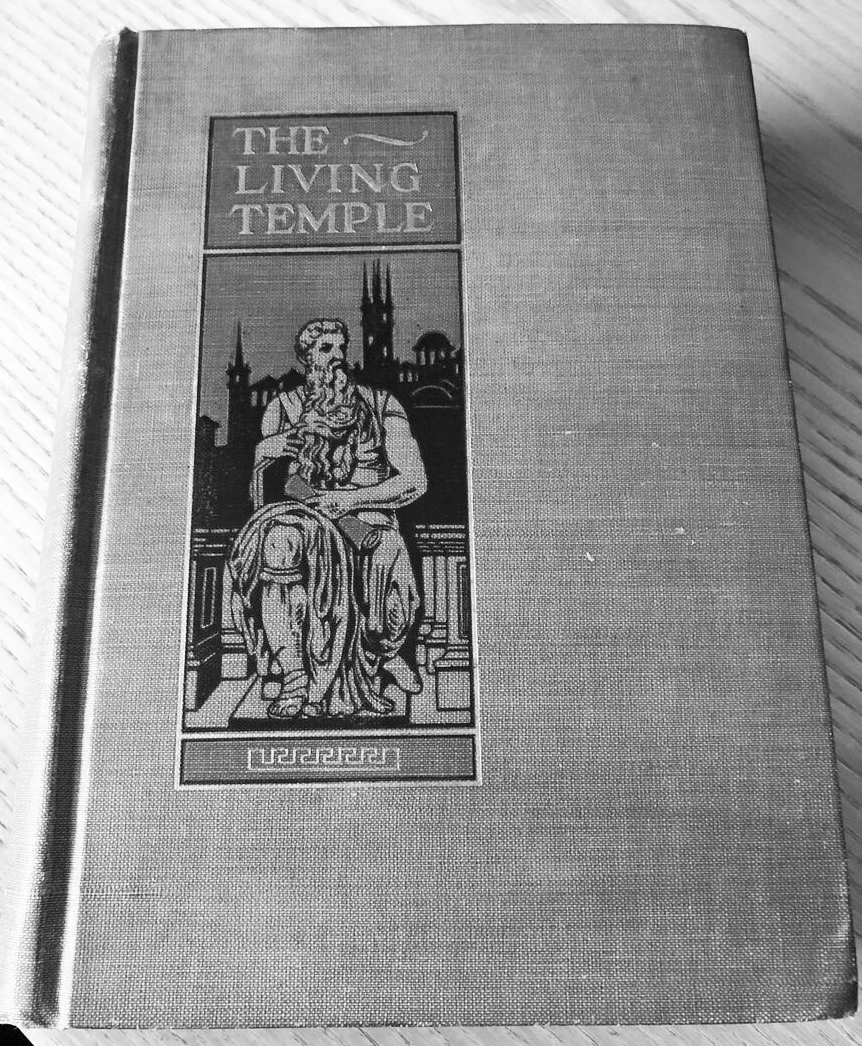
\includegraphics[width=1\linewidth]{images/TLT.jpg}
    \caption*{The Living Temple autorstwa dr. J. H. Kellogga, 1903.}
    \label{fig:tlt}
\end{figure}

Niektórzy ludzie uważają, że rozumienie osobowości Boga przez dr. Kellogga współgra z ich rozumieniem, choć są kuszeni, by sądzić, że to inne rzeczy są godne sprzeciwu w \textit{The Living Temple}. Poniższe dowody sugerują coś zupełnie przeciwnego. Istnieje list od dr. Kellogga do Williama C. White’a, w którym dr Kellogg proponuje \others{wycięcie kilku stron} z trzech tysięcy egzemplarzy \textit{The Living Temple} — właśnie tych stron zawierających \others{szczególnie kontrowersyjne treści, takie jak komentarz do 40. rozdziału Księgi Izajasza} i poglądy dotyczące \emcap{osobowości Boga} (strony, które przeczytaliśmy).

\others{Sanatorium posiada, jak się dowiedziałem, \textbf{dwa lub trzy tysiące książek, które zostały sprzedane}, ale które wróciły po tym, jak książka została potępiona. Pojawiło się pytanie, co z nimi zrobić. \textbf{Przyszło mi do głowy, że być może można by je uratować, \underline{wycinając kilka stron}, na których pojawiają się \underline{szczególnie kontrowersyjne treści}, takie jak \underline{komentarz do 40. rozdziału Księgi Izajasza}, który zapożyczyłem od A. T. Jonesa, oraz stronę, na której pojawia się niefortunny nagłówek «\underline{Osobowość Boga}», i wklejając strony zawierające jasne przedstawienie biblijnego poglądu na Boga jako osobę, przedstawionego w artykule starszego Haskella w «Review» kilka tygodni temu}. Te książki zostałyby sprzedane dawnym pacjentom, którzy bardzo domagają się tej książki na prezenty świąteczne...}[List dr. J. H. Kellogga do W. C. White’a; 6 grudnia 1903, Chicago.][https://174625.selcdn.ru/ellenwhite/EWhite/17226/17226.pdf]

Jaki jest prawdziwy problem z rozumowaniem w \textit{The Living Temple}? Zbadamy tę sprawę do samego sedna; na pierwszy rzut oka wyraźnie widzimy, że problemem jest odstąpienie od fundamentu naszej wiary — \emcap{Fundamentalnych Zasad} — w odniesieniu do \emcap{osobowości Boga} i tego, gdzie jest Jego obecność.

\egw{\textbf{Zostałam pouczona przez niebiańskiego posłańca}, że część rozumowania w książce «The Living Temple» jest niepoprawna i że \textbf{to rozumowanie sprowadziłoby na manowce} umysły tych, którzy nie są całkowicie utwierdzeni w \textbf{fundamentalnych zasadach} teraźniejszej prawdy. \textbf{Wprowadza to, co jest niczym innym jak spekulacją} w \textbf{odniesieniu do osobowości Boga i tego, gdzie jest Jego obecność}}[SpTB02 51.3; 1904][https://egwwritings.org/?ref=en\_SpTB02.51.3]

Dr Kellogg wprowadził myśl, która \egwinline{jest niczym innym jak spekulacją w odniesieniu do osobowości Boga}, przez co odstąpił od fundamentu naszej wiary — \emcap{Fundamentalnych Zasad}. Niezgodność między nauczaniem dr. Kellogga a \emcap{Fundamentalnymi Zasadami} znajduje się w pierwszym punkcie zasad, gdzie jesteśmy nauczani, że \others{Jest \textbf{jeden Bóg}, \textbf{osobowa, duchowa \underline{istota}}, \textbf{stwórca wszystkich rzeczy}, [...] i \textbf{wszędzie obecny przez swojego przedstawiciela, Ducha Świętego}. Ps 139:7}

Siostra White bezpośrednio ostrzegała nas przed poglądami wyrażonymi w \textit{The Living Temple} dotyczącymi \emcap{osobowości Boga}. Nie są one zgodne z pierwszym punktem \emcap{Fundamentalnych Zasad}, które były częścią fundamentu naszej wiary.

\egw{\textbf{Musiałam już napisać wiele na temat dziwnych doktryn i teorii wyrażonych w «The Living Temple». \underline{Gdyby te teorie zostały przyjęte przez nasz lud, silne filary naszej wiary i prawdy, które uczyniły Adwentystów Dnia Siódmego tym, czym są, zostałyby zmiecione}. Musiałam pokazać błędność tych doktryn, przedstawiając je \underline{jako rodzaj herezji czasów końca}. Słowo Boże mówi nam, że właśnie takie nauczanie \underline{będzie wprowadzane w tym czasie}}}[Lt250-1903.2; 1903][https://egwwritings.org/?ref=en\_Lt250-1903.2&para=9337.8]

Dziś jesteśmy świadkami powszechnego przyjęcia teorii Kellogga dotyczących \emcap{osobowości Boga}. Fakt, że pierwszy punkt \emcap{Fundamentalnych Zasad} nie jest już obecny w naszych wierzeniach, dowodzi, iż teorie Kellogga dotyczące \emcap{osobowości Boga} miały wpływ na kształtowanie naszych wierzeń.

\egw{Jeden po drugim przychodzą do mnie z prośbą o \textbf{wyjaśnienie stanowisk zajętych w «The Living Temple»}. Odpowiadam: «Są one niewytłumaczalne». \textbf{Wyrażone tam poglądy nie dają prawdziwego poznania Boga.} \textbf{W całej książce znajdują się fragmenty Pisma Świętego}. \textbf{Te fragmenty Pisma są przedstawione w taki sposób, że \underline{błąd wydaje się być prawdą}}. \textbf{Błędne teorie są przedstawione w tak ujmujący sposób, że jeśli nie zachowa się ostrożności, wielu zostanie wprowadzonych w błąd}}[SpTB02 52.1; 1904][https://egwwritings.org/?ref=en\_SpTB02.52.1&para=417.265]

Błąd jest przedstawiany jako prawda i wielu jest wprowadzanych w błąd.

Warto podkreślić, dla niektórych nieuważnych czytelników, że prawdziwy problem dr. Kellogga i jego książki \textit{The Living Temple} nie dotyczy Trójcy, lecz małego kroku, który wykonał, odchodząc od \emcap{fundamentalnych zasad}. Aby zrozumieć prawdziwy problem jego książki, błędem byłoby skupianie się na jej poglądach zbieżnych z doktryną o Trójcy. Zamiast tego powinniśmy skupić się na punkcie, który stanowił ten mały krok wykonany przez niego; a to wymaga głębokiego zrozumienia \emcap{Fundamentalnych Zasad}, tak jak mieli je nasi pionierzy. Kogo lepiej zapytać niż samych pionierów adwentyzmu?

\begin{titledpoem}

    \stanza{
        Bóg osobowy na tronie zasiada, \\
        Tak nasza Zasada Fundamentalna powiada. \\
        Wszędzie obecny przez Ducha swojego, \\
        To fundament wiary ludu Bożego.
    }

    \stanza{
        Lecz przyszły słowa, co mądre się zdały, \\
        I w nieświadomy umysł głęboko się wlały. \\
        Subtelna zmiana Kelloga, tak gładko przedstawiona, \\
        Była sidłem, w którym dusza została uwięziona.
    }

    \stanza{
        Błąd ubrany w prawdę pięknie się prezentuje, \\
        Gdy Pismo wykręcone zręcznie argumentuje. \\
        Mały krok od Zasad, które wyznawaliśmy, \\
        Wielki skok, przez który wiarę utraciliśmy.
    }

    \stanza{
        Fundamenty wiary stoją niewzruszone, \\
        Choć teorie nowe są wciąż przedstawione. \\
        Bóg Ojciec, osobowa duchowa istota, \\
        To prawda, której broni nasza wiara złota.
    }
    
\end{titledpoem}
